\capitolo{Controllo del Moto per Trasmissione Rigida Senza Gioco}
Nell'industria i controllori sono di tipo P, PI, quindi le valutazioni saranno su questi.
Il modello di riferimento è quello classico del sistema motore, riduttore, carico a cui si aggiunge l'espressione base del motore:
\[
\begin{cases}
    C_m(t) = J \AccAng(t) + f \VelAng(t) + C_e (t) \\
    C_m(t) = K_T i(t)
\end{cases}
\]

Che trasformata in Laplace diventa:
\[
\begin{cases}
    C_m(s)=(Js^2+fs)\theta(s) + C_e (s) \\
    C_m(s)=K_T I(s)
\end{cases}
\]

In cui sono state raggruppate tutte le varie inerzie, coefficienti di attrito e coppie legate a forze esterne.
Il sistema è a 1gdl.

\paragrafo{Schema Multi-Anello:}
In un sistema motore, riduttore, carico ci sono solitamente diversi anelli di controllo. Partendo dall'interno verso l'esterno ci sono gli anelli di: (tensione)\footnote{Nominato, ma non viene esaminato.} corrente, velocità e posizione.

\sottoparagrafo{Anello di corrente:}
L'anello di corrente è indipendente dalla meccanica; dipende dall'elettrica, dall'elettronica e dal controllo. Ha anche bande passanti caratteristiche ad alta frequenza \([kHz]\).

\sottoparagrafo{Anello di posizione:}
L'anello di posizione dipende: anello di velocità; trasduttore di posizione; controllo di posizione. In applicazioni tipiche ha banda passante inferiore i \(50 Hz\). 

\paragrafo{Feedback vs Feedforward:}
Nella trattazione classica dei controlli si tende a valutare soprattutto il sistema con feedback (catena chiusa), però tende a limitare le prestazioni. Un approccio più flessibile utilizza un feedback ben sintonizzato e un feedforward (catena aperta) basato sulla conoscenza (approssimata) del sistema fisico e del modello, che si traduce in una stima (nota a priori) di corrente\footnote{Nel caso dell'anello di velocità.} richiesta per la movimentazione.

\sezione{Anello di Velocità}
\import{Immagini/}{modello_complessivo}

L'anello di velocità dipende da: anello di corrente; meccanica; trasduttori di velocità; controllore di velocità.
Tipicamente ha bande passanti sul centinaio di \([Hz]\).

\sottosezione{Modello Semplificato 1}
Lo schematico in figura è quello completo, tuttavia in prima analisi conviene fare delle approssimazioni:
\begin{itemize}
    \item Coppie esterne vengono trascurate (valido per sovrapposizione degli effetti)
    \item Non utilizzo feedforward
    \item Trasduttore ideale, la misura non ha ritardi o errori, è come se il blocco relativo fosse 1
    \item Anello di corrente ideale, la corrente erogata, è come se il blocco relativo fosse 1
\end{itemize}

\import{Immagini/}{modello_semplificato_1}

\sottosottosezione{Controllo proporzionale}
Considerando il modello semplificato e l'utilizzo di un controllo di tipo proporzionale, ottengo che la funzione di trasferimento del sistema a catena chiusa è 
\[W(s)=\frac{K_{pv}K_T}{K_{pv}K_T+f}\frac{1}{1+s\frac{J}{f+K_{pv}+K_T}}\]
dove \(\tau = \frac{J}{f+K_{pv}+K_T}\) è la costante di tempo\footnote{Nota bene: si può parlare di costanti di tempo solo per sistemi del primo ordine.}.

\paragrafo{Banda passante:}
In un sistema del primo ordine la banda passante è data da \(\omega_B=\frac{1}{\tau}\), tuttavia considerando trascurabile l'attrito risulta \(\omega_B\simeq \frac{K_{pv}K_T}{J}\). Quest'ultima relazione permette facilmente di sintonizzare il controllore invertendo \(K_{pv}=\frac{\omega_B J}{K_T}\).

\paragrafo{Errore a regime:}
Per un sistema del primo ordine il guadagno in continua/regime è dato da \(\frac{K_{pv}K_T}{K_{pv}K_T+f}<1\), che è necessariamente minore di 1, ossia l'errore a regime non è nullo. Questo è molto negativo. Non potendo impostare un guadagno proporzionale infinito, occorre necessariamente valutare un controllore di altro tipo che permetta di ottenere un errore a regime nullo, di modo da avere un guadagno in continua unitario.

\sottosottosezione{Controllo Proporzionale Integrale}
Un controllore PI è del tipo \(C_V(s)=K_{pv}\frac{1+sT_{iv}}{sT_{iv}}\), per cui il sistema a catena chiusa diventa 
\[W_v(s)=\frac{K_{pv}K_T(1+sT_{iv})}{s^2T_{iv}J + sT_{iv}(f+K_{pv}K_T)+K_{pv}K_T}\]
Come era voluto, il sistema così ottenuto ha guadagno in continua unitario.
Però aumenta il numero di poli, diventa di secondo ordine\footnote{Passando da un primo a un secondo ordine occorre fare attenzione per una serie di implicazioni; fare riferimento a quanto presente in appendice \ref{sistemi_ordine_2}.} e viene aggiunto uno zero reale, che ha anch'esso forti implicazioni. Tuttavia il grado relativo rimane 1.

\paragrafo{Effetto dello zero reale:}
Per valutare bene l'effetto dello zero nel sistema a catena chiusa adotto una parametrizzazione:
\[\frac{1+\frac{s}{\alpha \xi \omega_n}}{\left(\frac{s}{\omega_n}\right)^2+\frac{2\xi}{\omega_n}s+1}\]
Utilizzare \(\alpha\) permette di valutare dove si trova lo zero rispetto i poli del sistema
\[
\begin{cases}
\alpha >> 1 \text{ \ zero in alta frequenza} \\
\alpha \simeq 1 \text{ \ zero vicino ai poli} \\
\alpha << 1 \text{ \ zero in bassa frequenza}
\end{cases}
\]
In particolare si nota come la presenza dello zero vada a incrementare la sovraelongazione.

\textbf{La sovraelongazione dipende da \(\xi\) e dalla posizione dello zero.} Di seguito un immagine con relazione tra picco di sovraelongazione \(M_p\) e posizione dello zero \(\alpha\).

\begin{figure}[h]
    \centering
    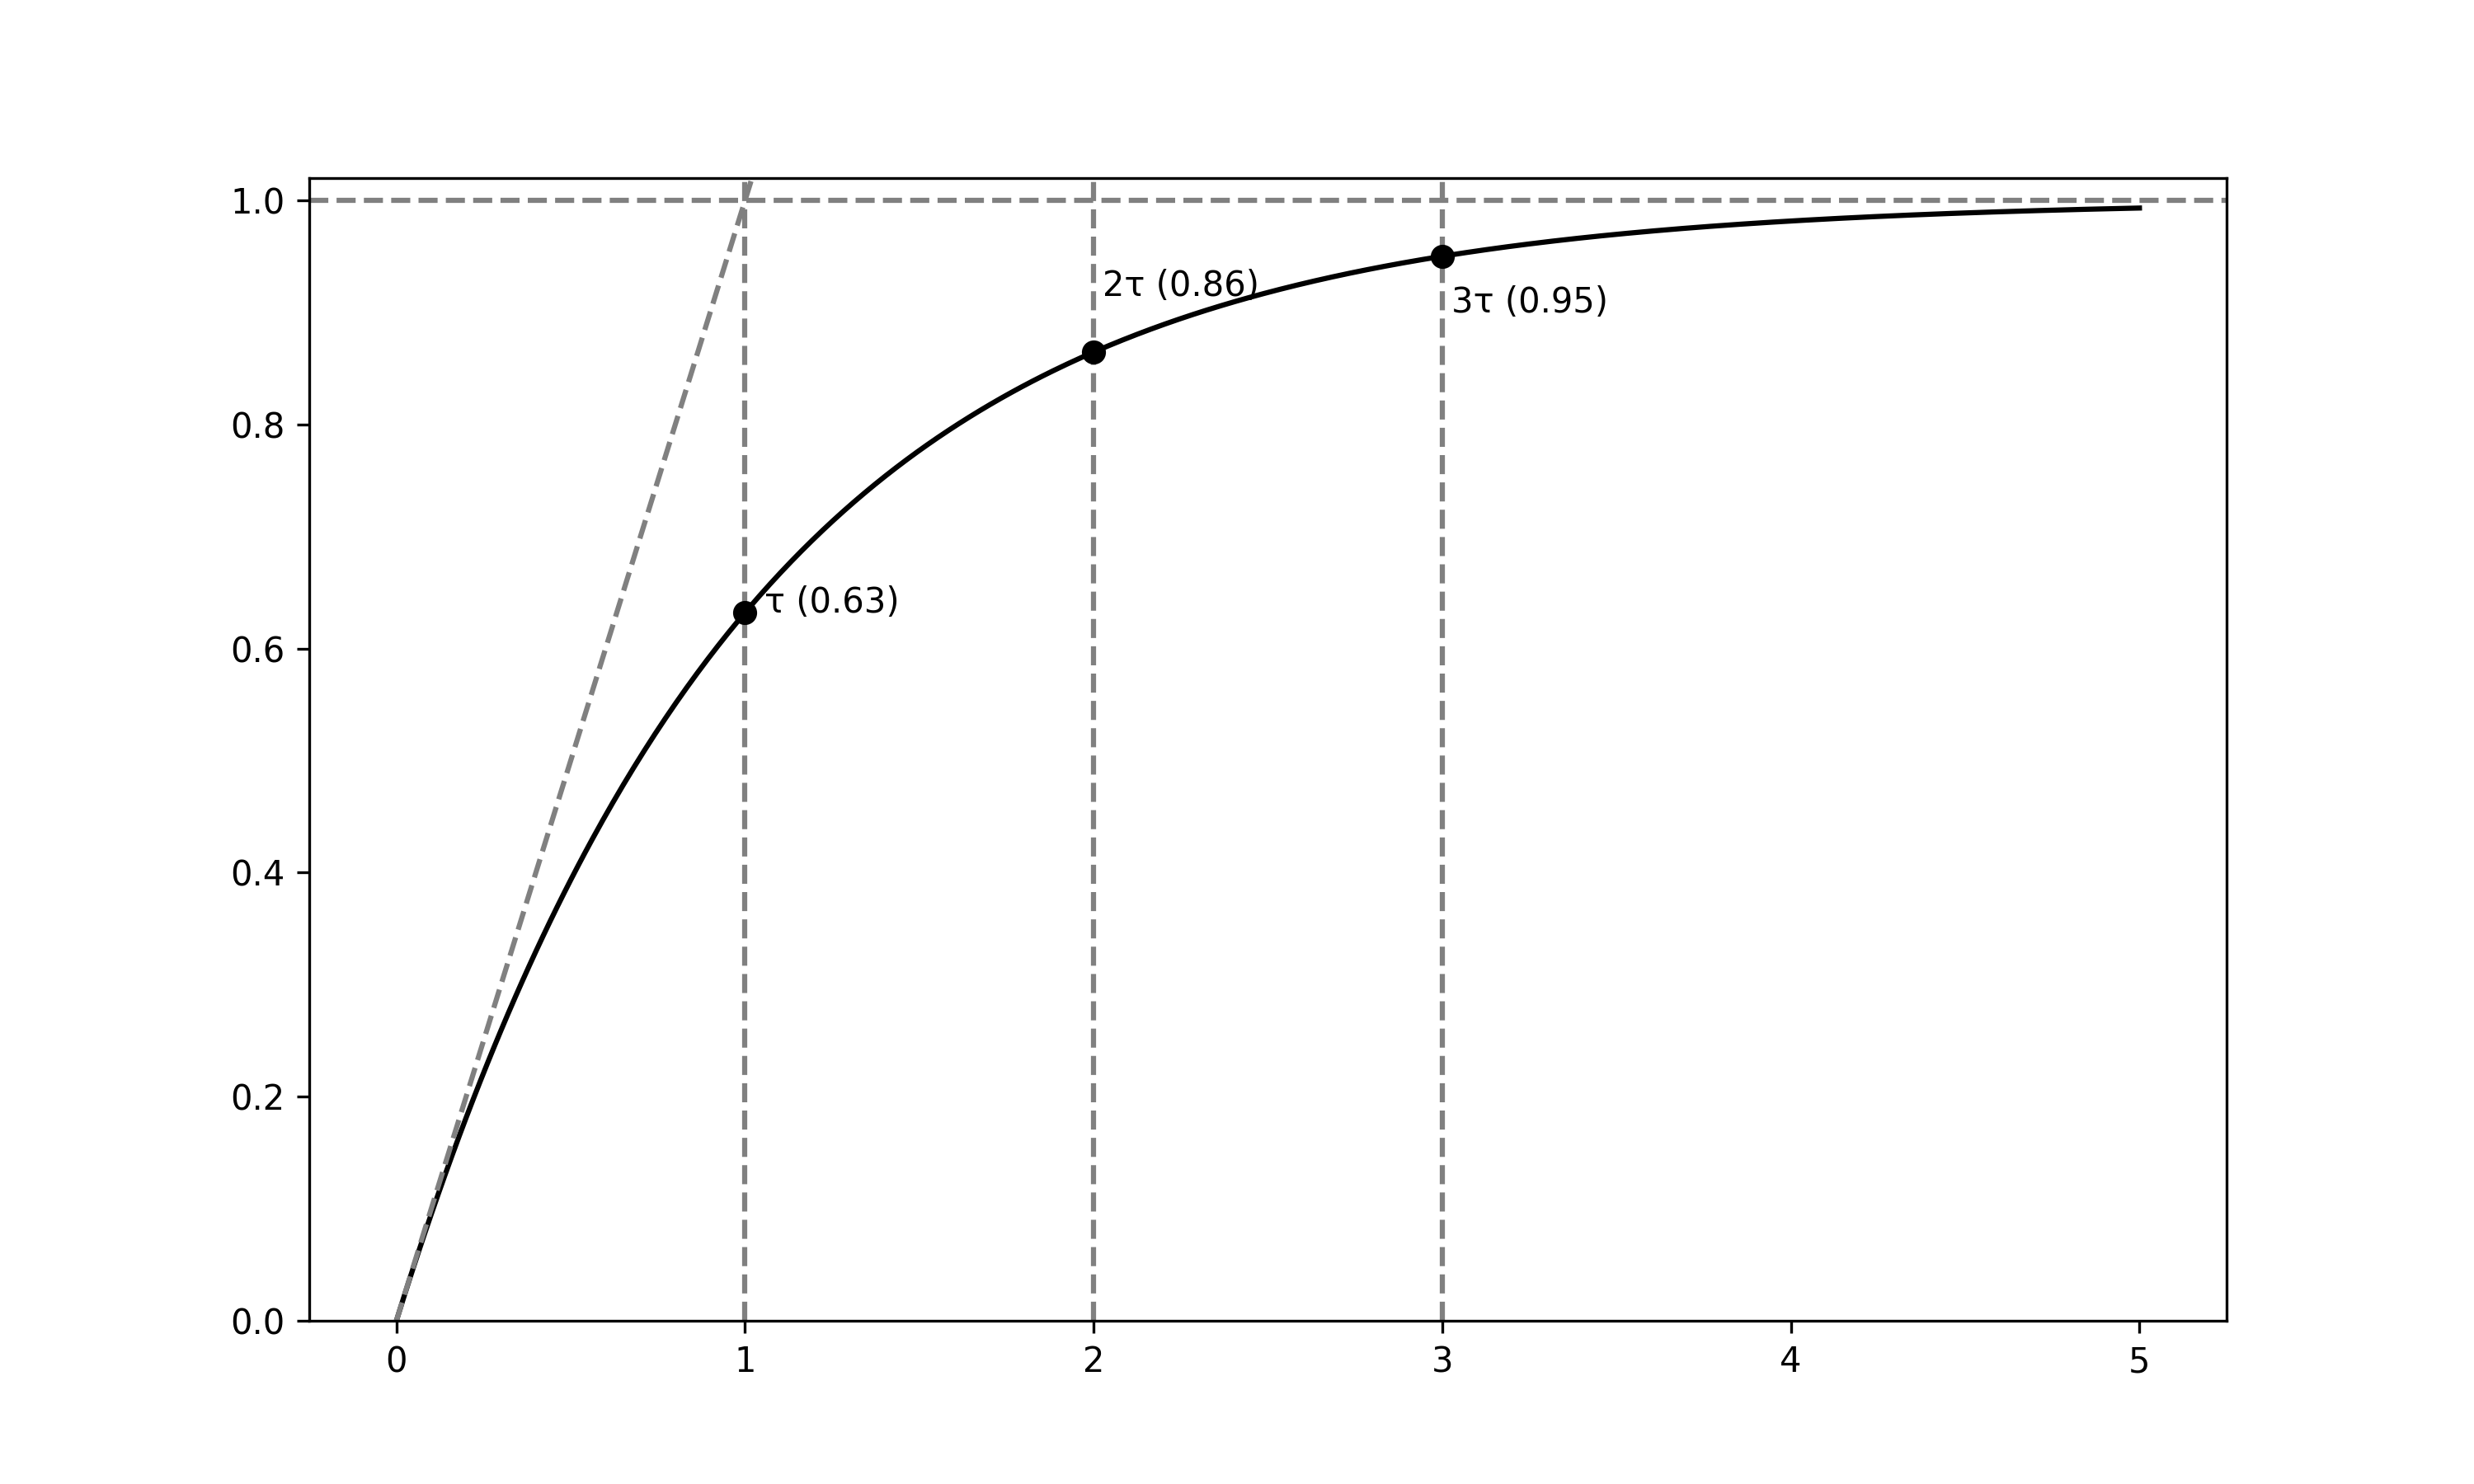
\includegraphics[width=0.45\textwidth]{Immagini/risposta_gradino_ord1_tempo.png}
    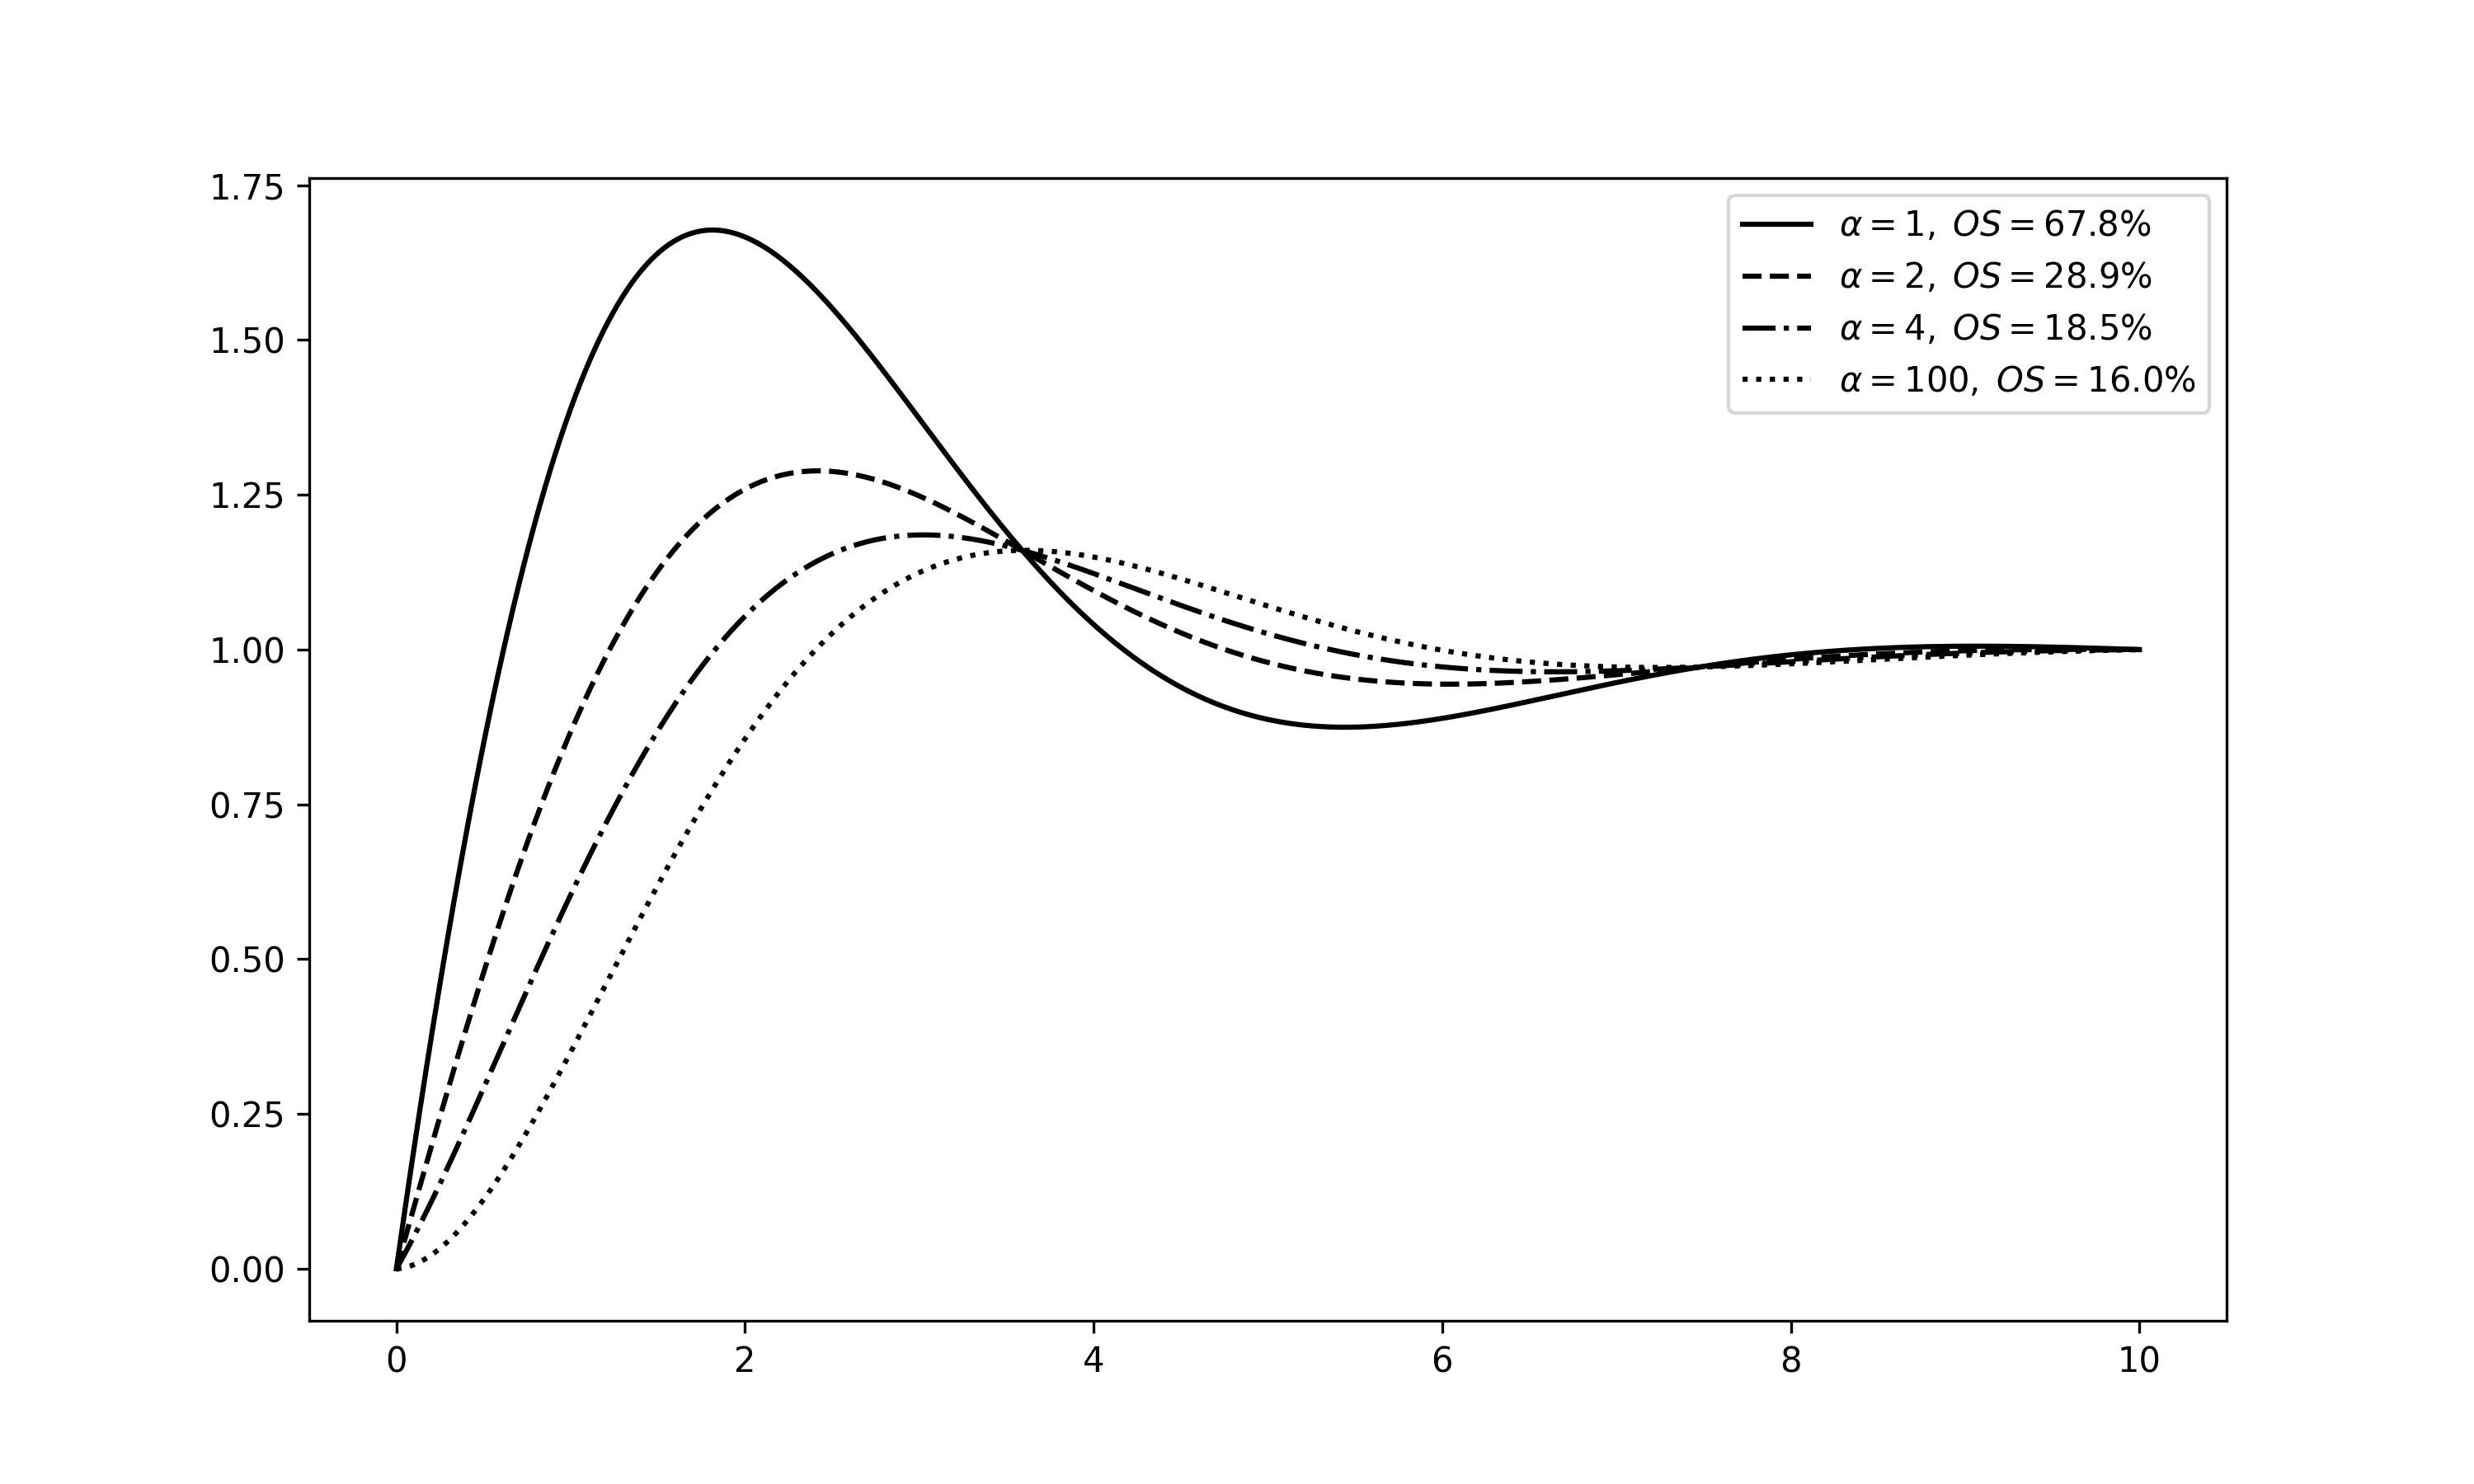
\includegraphics[width=0.45\textwidth]{Immagini/influenza_zero_su_sovraelong.png}
    \caption{Risposta al gradino di sistema di ordine 1 (sx); \(M_p(\alpha)\) in risposta al gradino (dx)}
\end{figure}

\sottoparagrafo{Scomposizione sovraelongazione poli e zero:}
A partire dal sistema a catena chiusa, vado a scomporre la componente legata al sistema del secondo ordine dal resto, cioè un sistema del secondo ordine derivato \(H(s)=\frac{1}{\left(\frac{s}{\omega_n}\right)^2+\frac{2\xi}{\omega_n}s+1} + \frac{1}{\alpha \xi \omega_n}\frac{s}{\left(\frac{s}{\omega_n}\right)^2+\frac{2\xi}{\omega_n}s+1}\), che nel tempo diventa \(h(t)=h_{2 ord}(t) + \frac{1}{\alpha \xi \omega_n} \derivata{h_{2 ord}(t)}{t}\).

Nella risposta al gradino avrò una componente legata alla risposta al gradino del sistema del secondo ordine e una componente legata alla risposta all'impulso\footnote{Impulso che è la derivata del gradino.} del sistema del secondo ordine.
\begin{itemize}
    \item Se cala lo smorzamento, a parità del resto, la sovraelongazione aumenta per effetto dello zero: \(\downarrow \xi \ \uparrow M_p\)
    \item Se \(\alpha >>1\) l'effetto legato allo zero diventa trascurabile
    \item Se \(\alpha <<1\) l'effetto legato allo zero è tanto più severo tanto è minore lo smorzamento
\end{itemize}

Quindi per attenuare la sovraelongazione conviene:
\begin{itemize}
    \item Posizionare gli zeri ad alta frequenza \(>> \xi \omega_n\)
    \item Se \(\xi << 1\) aumenta la sensibilità allo zero quindi lo zero va portato ancora  a più alta frequenza
    \item Se non è possibile intervenire su \(\alpha, \xi\), occorre intervenire sulla legge di moto
\end{itemize}

\begin{figure}[h]
    \centering
    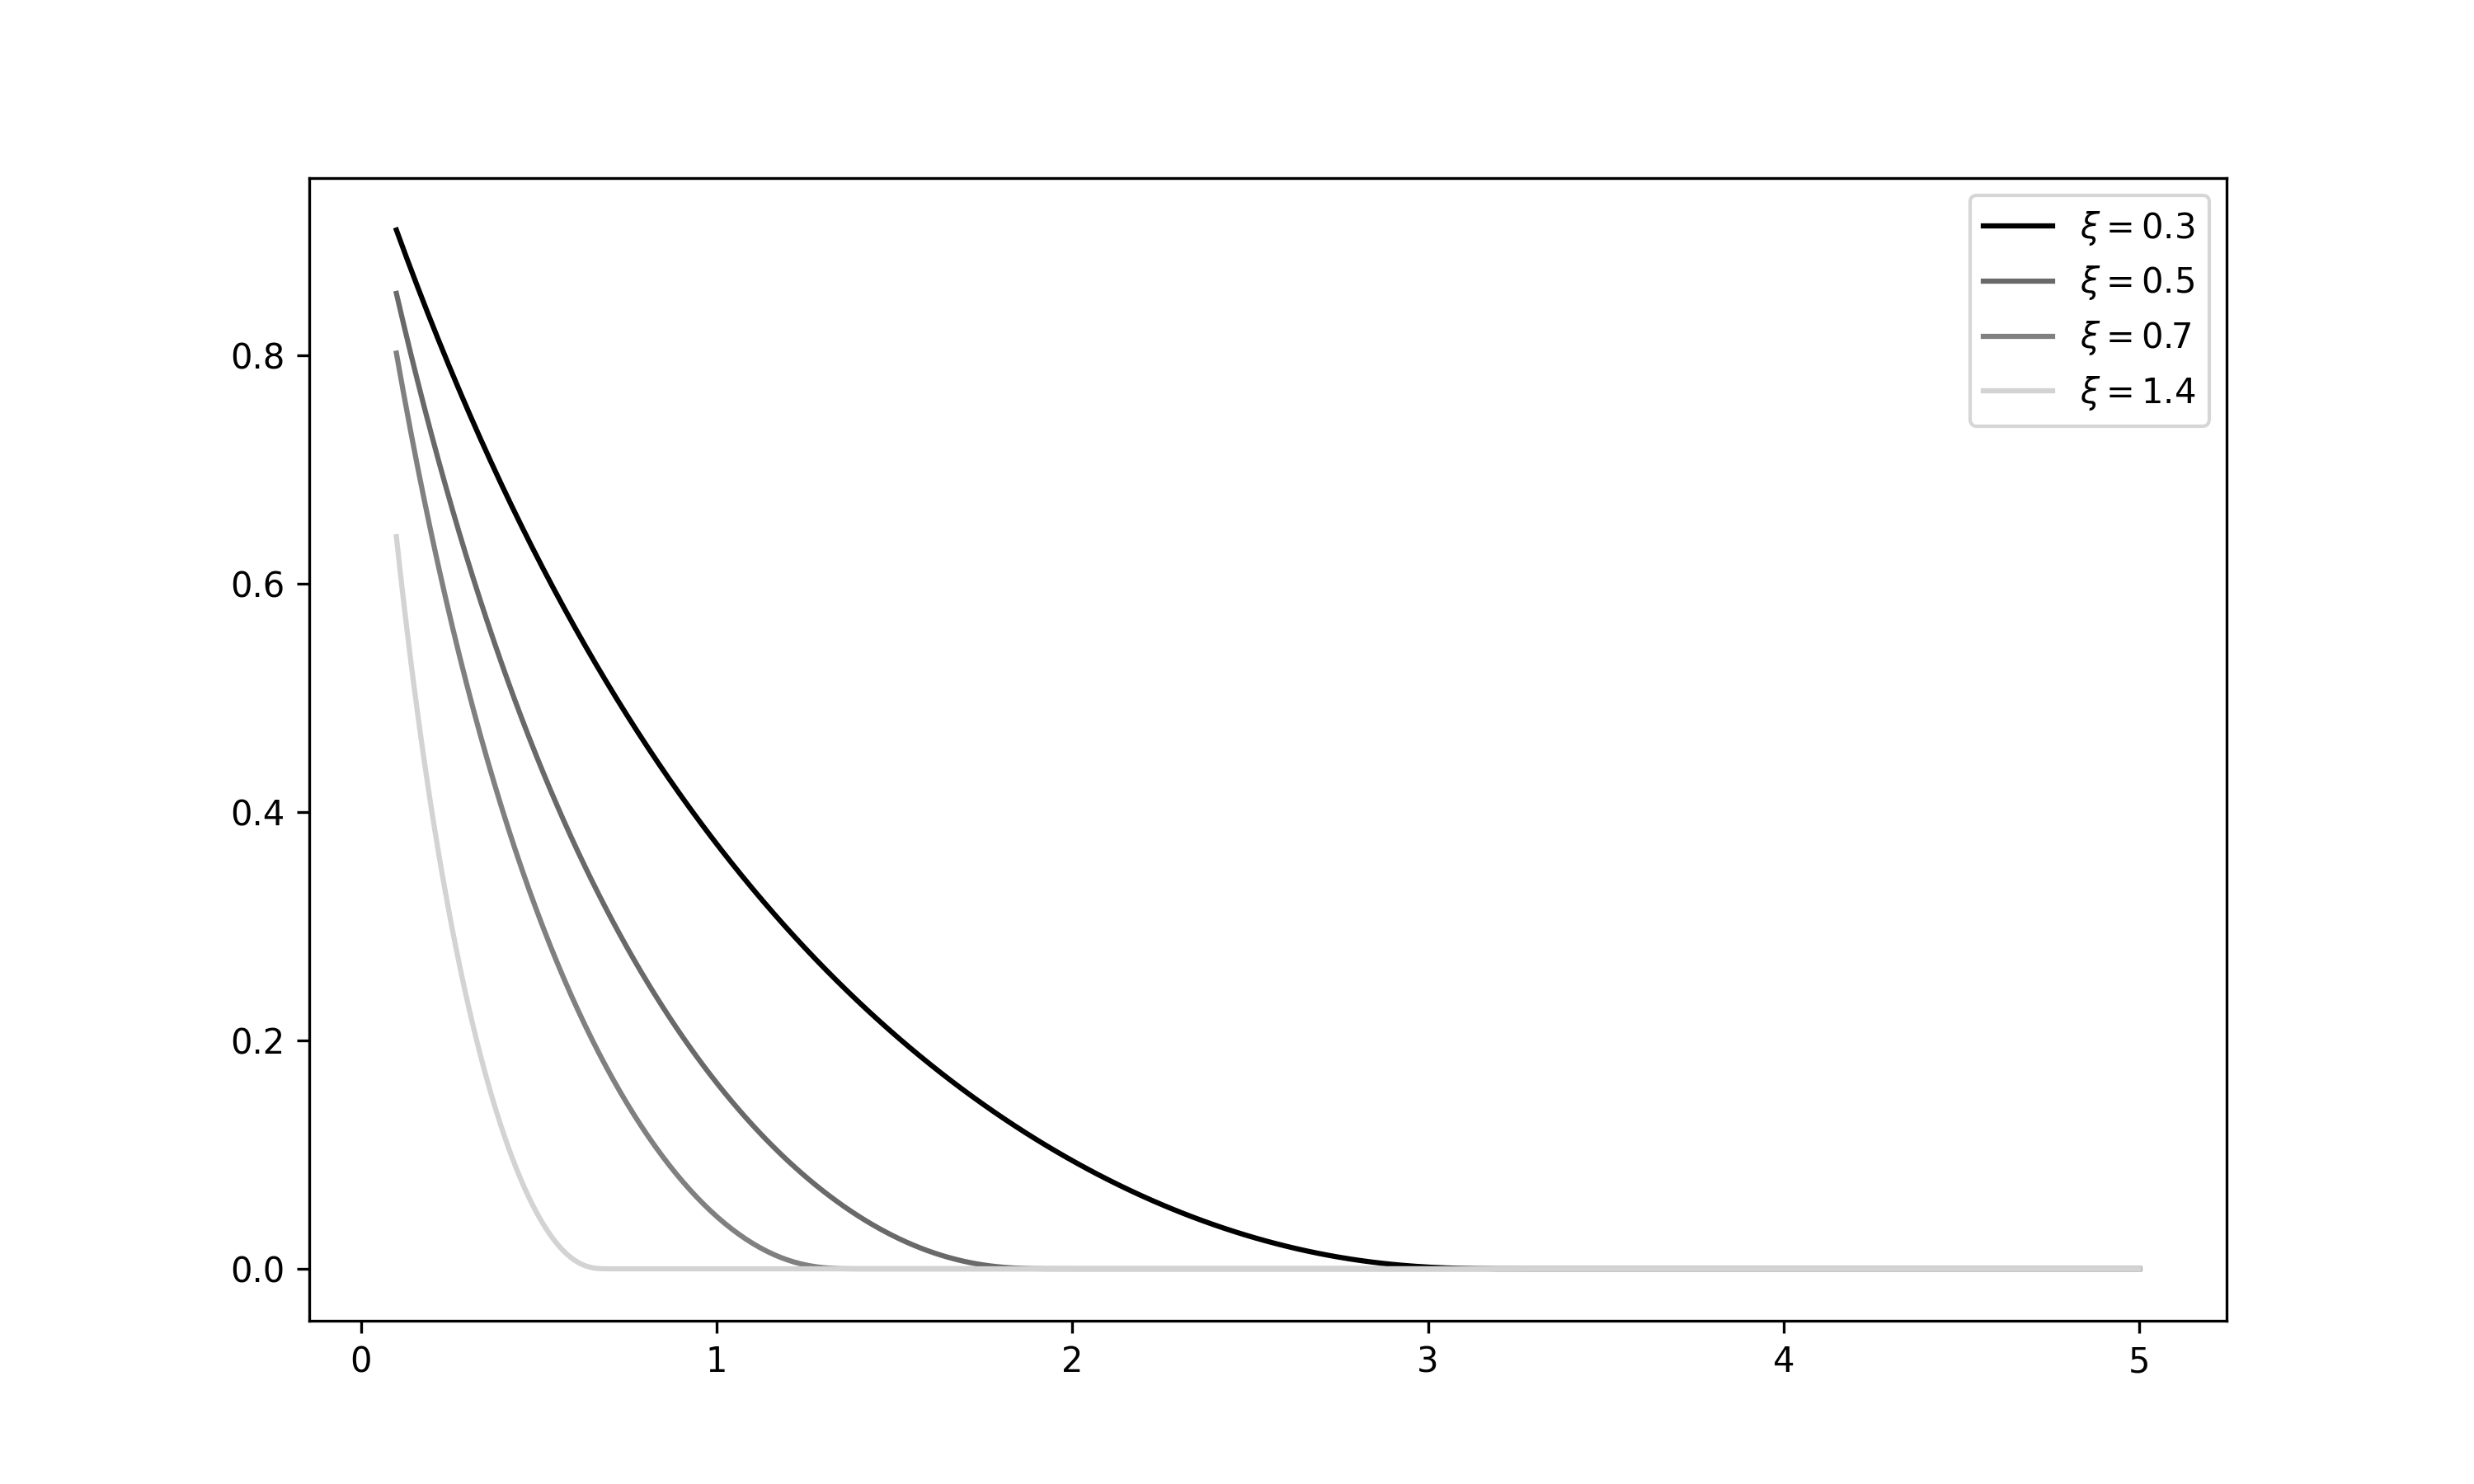
\includegraphics[width=0.6\textwidth]{Immagini/relazione_sovraelongazione.png}
    \caption{Relazione tra \(\alpha\) e \(M_p\)}
\end{figure}

\paragrafo{Banda passante:}
La banda passante di un sistema con controllore proporzionale è data da \(\omega_{b,v}=\frac{K_{pv}K_T}{J}\).
Riscrivendo la funzione di trasferimento per il controllore PI come visto per sistemi massa molla smorzatore \(W(s)=\frac{K_{pv}K_T(1+sT_{iv})}{s^2M_{eq} + s C_{eq} + K_{eq}}\), si ottengono come poli del sistema \(S_{1,2}=\frac{-C_{eq}\pm\sqrt{C_{eq}^2-4M_{eq}K_{eq}}}{2M_{eq}}\). Il fattore di smorzamento vale \(\xi = \frac{C_{eq}}{2\sqrt{M_{eq}K_{eq}}}=\frac{\sqrt{T_{iv}}}{2}\sqrt{\frac{K_{pv}K_T}{J}}\), dove la banda passante del sistema valeva per controllore proporzionale \(\omega_{b,v}=\frac{K_{pv}K_T}{J}\), quindi \(\xi=\frac{\sqrt{\omega_{b,v}T_{iv}}}{2}\).
Lo zero del PI è in corrispondenza di \(\frac{1}{T_{iv}}\), invertendo l'espressione di \(\xi\), si può riscrivere \(\frac{1}{T_{iv}} = \frac{\omega_{b,v}}{4\xi^2_{des}}\), ossia effettuando una opportuna scelta di fattore di smorzamento (\(\xi \in [0.7\div 1.4]\)  circa), la banda passante è ad un fattore 4 rispetto lo zero del PI, ossia la pulsazione di banda passante si ha quando l'effetto dell'integrale è già esaurito, quindi vale ancora la relazione della banda passante ricavata per controllore P:
\[\omega_{b,v}=\frac{K_{pv}K_T}{J}\]

\paragrafo{Approccio tipico alla risoluzione:}
Dati limiti e specifiche sulla banda, si definisce una banda passante desiderata, si ricava il coefficiente proporzionale \(K_{pv}\), vanno aggiunte specifiche sullo smorzamento, quindi si ricava \(T_{iv}\).

\sottosottosezione{Legge di Moto}
A leggi di moto più dolci si associano sovraelongazioni legate allo zero più trascurabili. A leggi di moto non dolci si associano sovraelongazioni legate allo zero maggiori.

L'utilizzo della finestratura (tempo finito) e la discontinuità in accelerazione, portano ad avere infinite armoniche. 
Tutto ciò che viene attenuato dalla banda passante comporta distorsione della legge nel tempo, tendendo ad addolcire la legge, eliminando le discontinuità. Questo effetto è più rilevante per leggi non dolci. Tuttavia, in una RtR, perdere armoniche porta a non ottenere arresto all'istante finale.

\paragrafo{Esempi:}
In termini di leggi di moto la risposta al gradino è non dolce, perciò gli effetti delle sovraelongazioni sono particolarmente acuiti.

\begin{figure}[h]
    \centering
    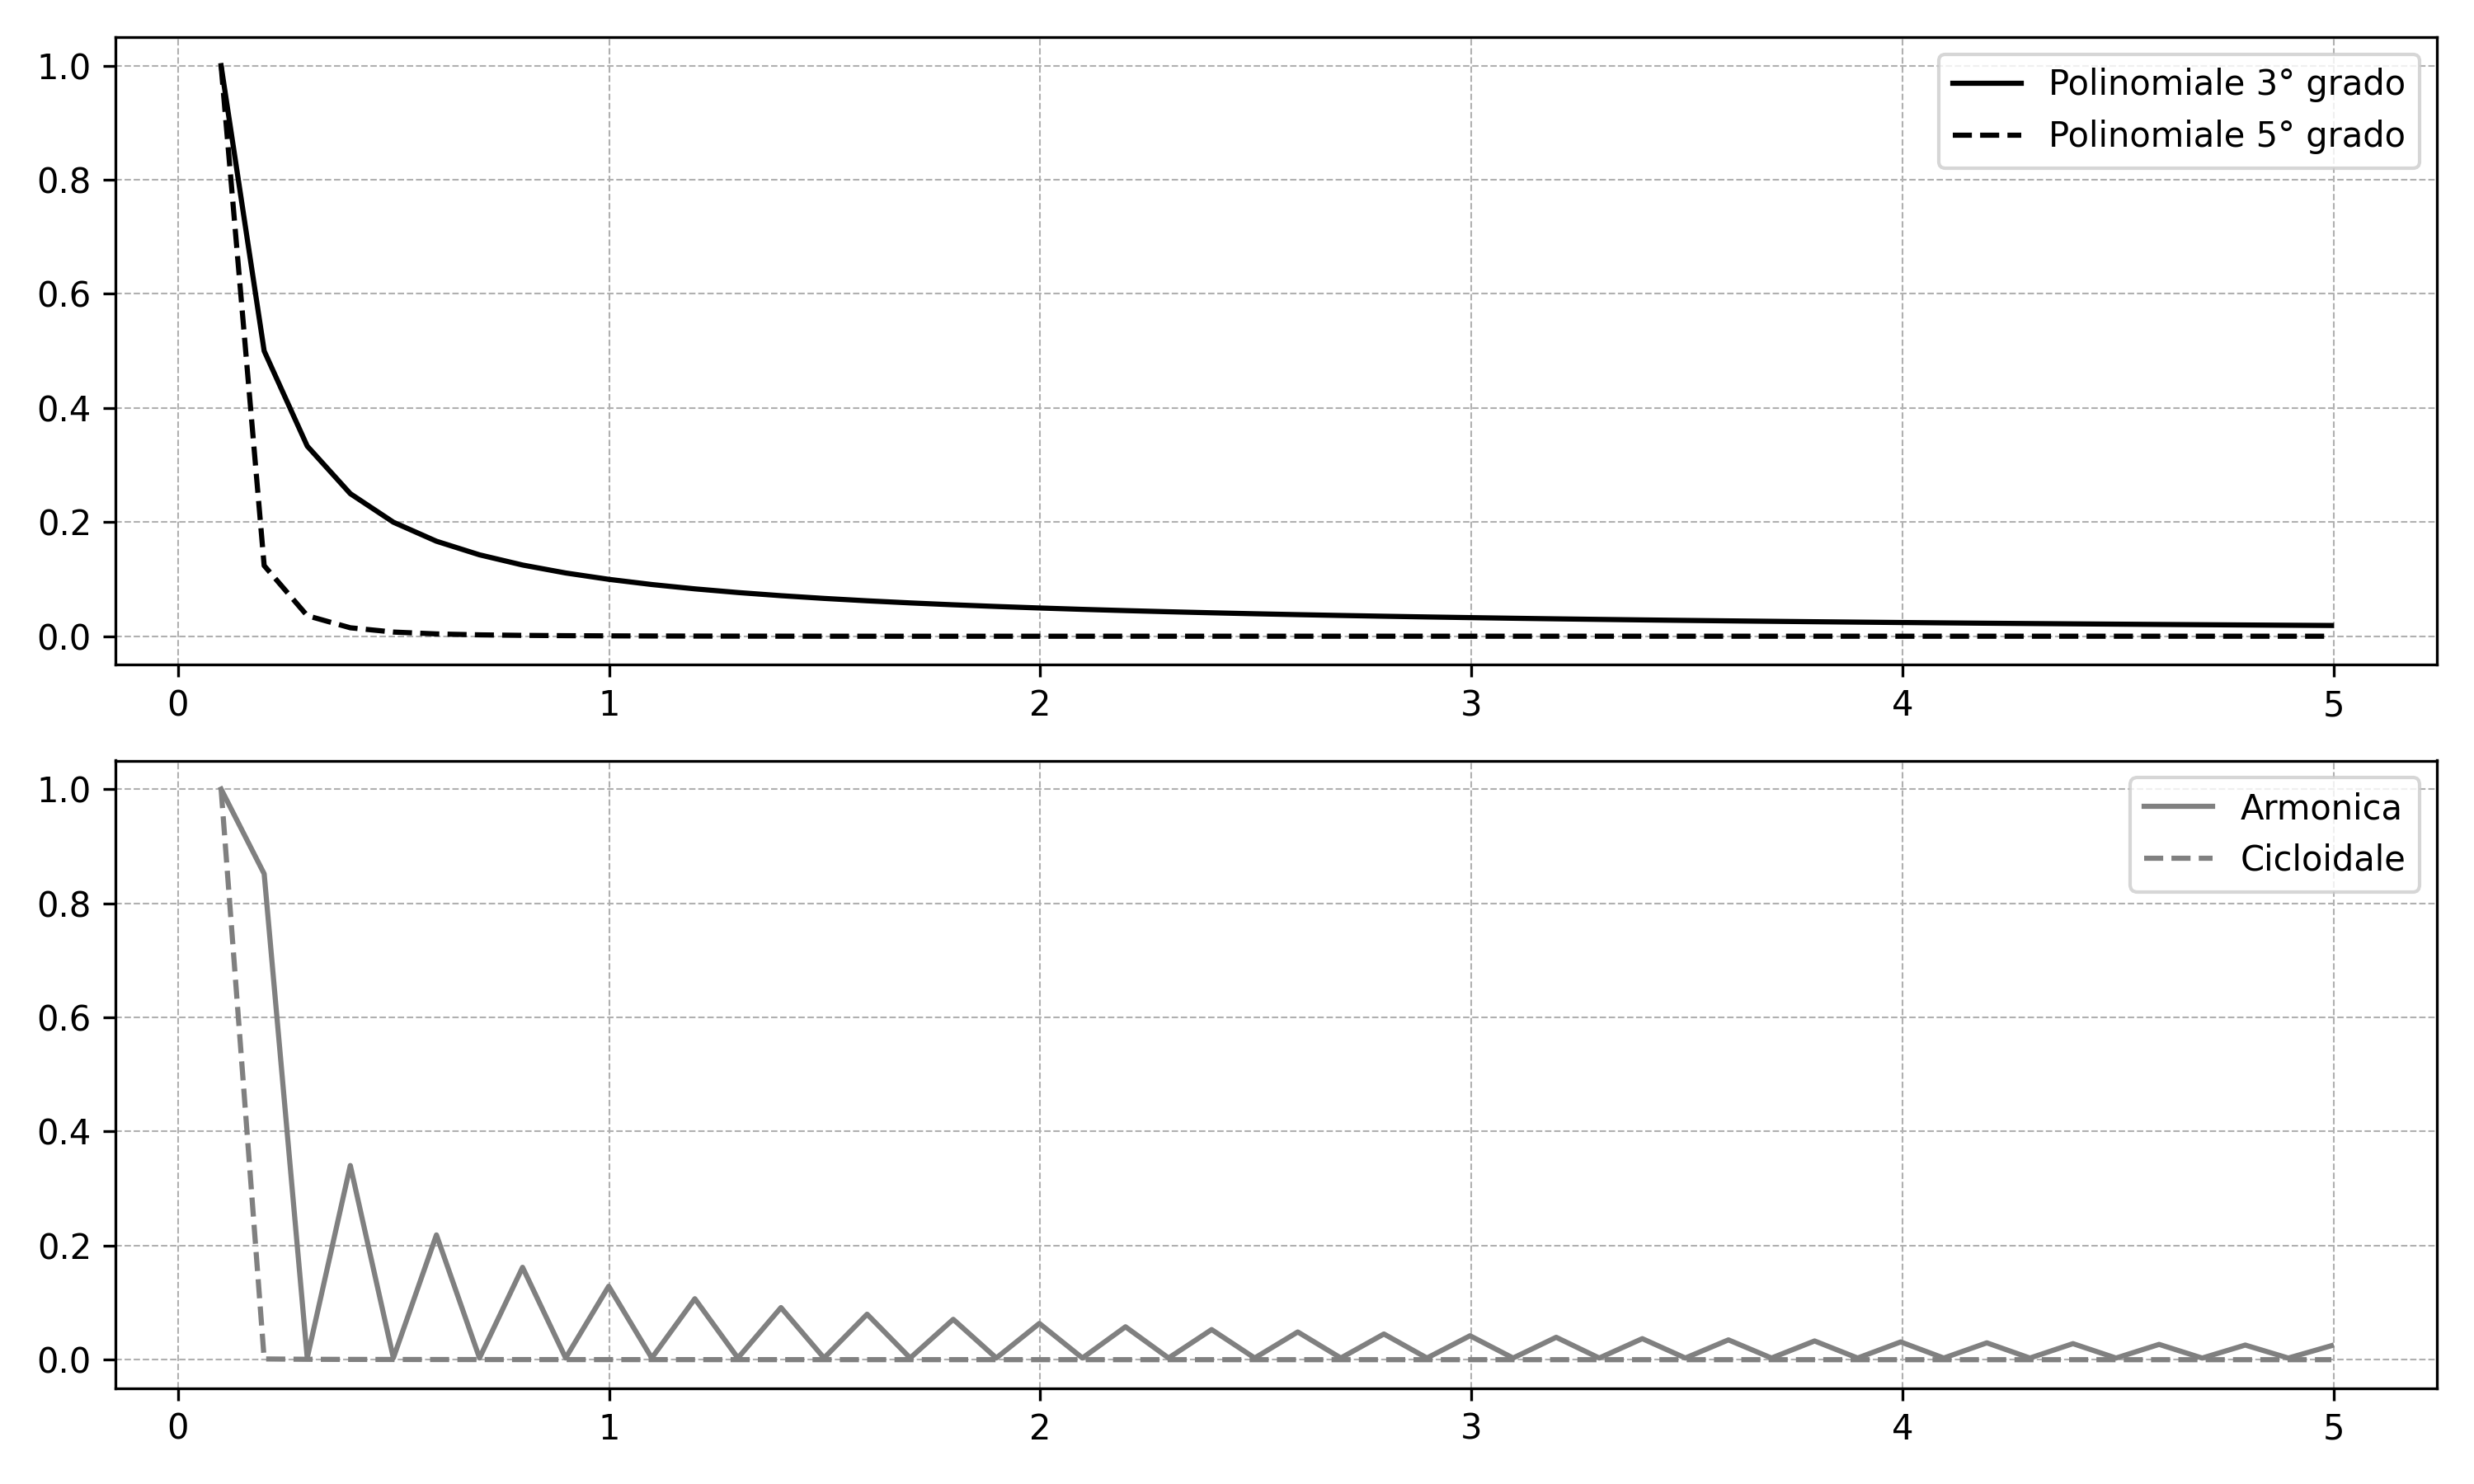
\includegraphics[width=0.6\textwidth]{Immagini/fft_leggi_di_moto.png}
    \caption{FFT delle principali leggi di moto}
\end{figure}

\paragrafo{Riduzione del tempo di moto:}
La riduzione del tempo di moto peggiora gli effetti di distorsione perché: le armoniche aumentano di frequenza, perciò è più facile vengano attenuate; inoltre le singole armoniche vedono un incremento in termini di ampiezza \(\propto \frac{1}{T^2}\).

\sottosezione{Modello semplificato 2}
A partire dal modello semplificato 1, vado a considerare anche l'anello di corrente e il trasduttore.
La funzione di trasferimento del sistema a catena aperta diventa: \(L_v(s)=C_v(s)W_I(s)K_T \frac{1}{sJ+f}H_{T_v}(s)\).

In prima approssimazione considero di introdurre i due elementi come sistemi del primo ordine: \(W_I(s) = \frac{1}{\frac{s}{\omega_I}+1}\) e \(H_{T_v}(s) = \frac{1}{\frac{s}{\omega_{T_v}}+1}\).

Un tipico ordine di grandezza è \(\frac{f}{J} < \frac{1}{T_{iv}} << \omega_{tv} < \omega_I\), la pulsazione del trasduttore di velocità e la quella dell'anello di corrente potrebbero essere scambiati.

Un aspetto da tenere bene a mente è la relazione di proporzionalità quasi lineare tra sovraelongazione e fattore di smorzamento\footnote{\(\xi \simeq \frac{m_\phi^\circ}{100^\circ}\)}: \(\uparrow \mathbf{m_\phi} \ \leftrightarrow \ \uparrow \boldsymbol{\xi}\).

\paragrafo{Valutazione su margine di fase:}
Dalla stabilità di Bode, noti i due strumenti del margine di fase e margine di guadagno, sapendo che portano a fare ragionamenti simili, per semplicità di trattazione verrà utilizzato il margine di fase\footnote{Vedi appendice \ref{CriterioBode}}.
In generale conviene cercare di tenersi lontano da margini di fase bassi (cui si associano smorzamenti equivalenti bassi), preferendo margini maggiori. La zona da preferire in questo modello è quella compresa tra \(\frac{1}{T_{iv}}\) e \(\min{\omega_{tv},\omega_I}\) in cui il margine di fase tende a \(90^\circ\). Assolutamente da evitare è la zona terminale, oltre \(\omega_I\) avente margine di fase negativo.

\sottosottosezione{Effetto di Kpv}
Fissato\footnote{Viene fatto unicamente per fare delle valutazioni, \(K_{pv}, T_{iv}\) vanno scelti in combinazione. {\color{red}{Vanno effettivamente scelti in combinazione?}}} \(T_{iv}\), variare \(K_{pv}\) porta a traslazione della curva del modulo (la fase resta invariata), perciò varia la pulsazione di attraversamento \(\omega_a\) e quindi varia la stabilità del sistema a catena chiusa.

\begin{figure}[h]
    \centering
    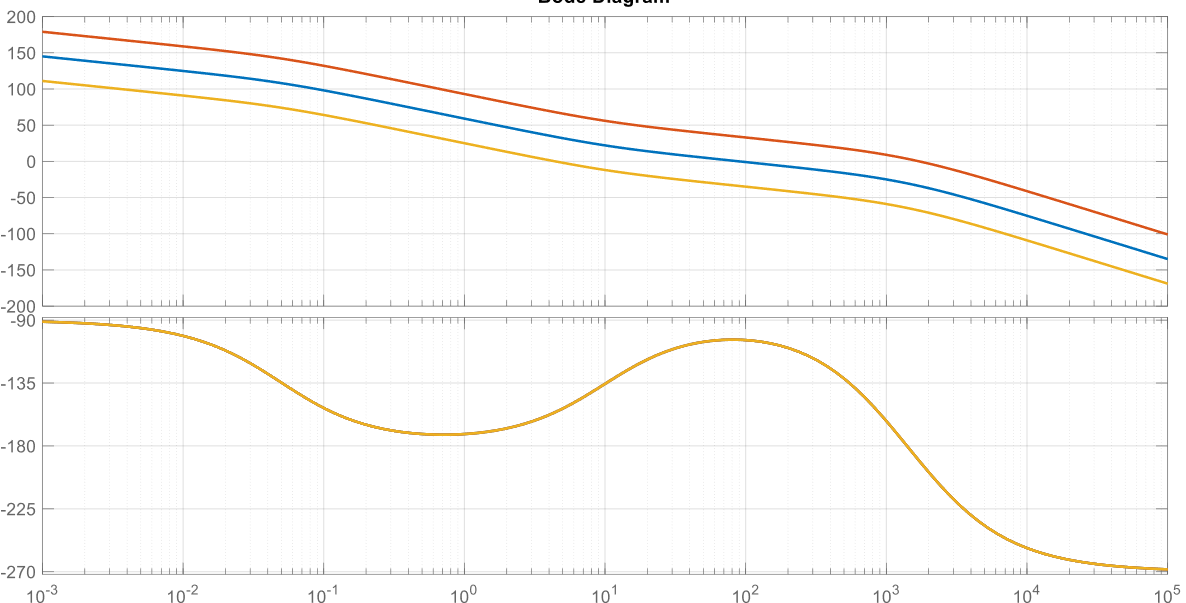
\includegraphics[width=0.6\textwidth]{Immagini/anello_aperto_anello_corrente.png}
    \caption{Modulo e fase di \(L_v(s)\)}
\end{figure}

\paragrafo{Logica di sintesi del controllore:}
La scelta di \(K_{pv}\) viene effettuata in modo tale da avere \(\omega_a \in \left[\frac{1}{T_{iv}}, \omega_{tv}\right]\) e \(\max{m_\phi} \simeq 90^\circ\), cercando di migliorare la robustezza. Si potrebbe privilegiare velocità di risposta e quindi valutare margini di fase minori.

\sottosottosezione{Stima di pulsazione di attraversamento per massimizzazione margine di fase}
Per la stima della pulsazione di attraversamento in corrispondenza del massimo margine di fase conviene utilizzare un modello semplificato, che permette di ottenere una buona precisione del calcolo, anche trascurando l'anello di corrente.

\paragrafo{1 - Trascurando l'anello di corrente:}
Considerando \(W_I(0)=1, \omega_I\rightarrow \infty\) e fissato \(T_{iv}\), si ottiene che la zona di interesse, \(\left[\frac{1}{T_{iv}}, \omega_{tv}\right]\), è simmetrica in fase (perché parte da \(-180^\circ\) e termina in \(-180^\circ\)),  perciò è possibile calcolare la pulsazione di attraversamento ottima utilizzando il metodo dell'ottimo geometrico\footnote{La fase è simmetrica nell'intervallo, tuttavia l'asse delle ascisse è logaritmico, perciò non si può fare una media come metà della somma dei valori di estremo.} \(\omega_{a,opt} = \sqrt{\frac{1}{T_{iv}}\omega_{tv}}\).

\paragrafo{2 - Considerando l'anello di corrente:}
Considerare l'anello di corrente porta differenze solo per frequenze "alte", per \(\omega>\frac{1}{T_{iv}}\), in particolare calano il valore massimo del margine di fase e la pulsazione cui si verifica. Unisco le pulsazioni ad alta frequenza in un unico contributo equivalente \(T_{eq}=\frac{1}{\omega_{tv}}+\frac{1}{\omega_I}\). Questo valore può essere utilizzato per valutare la pulsazione di attraversamento ottima \(\omega_{a,opt} = \sqrt{\frac{1}{T_{iv}}\frac{1}{T_{eq}}}\), che sarà paragonabile a quanto ottenuto nel caso precedente.

\paragrafo{3 - Considerando il tempo di campionamento dell'anello di velocità:}
Il controllore dell'anello di velocità ragiona in tempo discreto, tuttavia il sistema di interesse è quello fisico che lavora in tempo continuo. Tuttavia tra i due mondi c'è un legame, in particolare passanto da tempo discreto a tempo continuo si va ad introdurre un ritardo, che può essere approssimato con una funzione del tipo\footnote{Il ritardo in Laplace è rappresentato con un esponenziale, che tuttavia è scomodo da utilizzare, si utilizza quindi una forma approssimata.} \(H_{zoh}(s) \simeq \frac{1}{1+s\frac{T_c}{2}}\). In modo simile al precedente si può definire un contributo equivalente \(T_{eq}=\frac{1}{\omega_{tv}}+\frac{1}{\omega_I}+\frac{T_c}{2}\), da cui, come prima \(\omega_{a,opt} = \sqrt{\frac{1}{T_{iv}}\frac{1}{T_{eq}}}\), che sarà paragonabile a quanto ottenuto nel caso 1.

\paragrafo{4 - Trasduttore modellato con 2 poli reali:}
Un ulteriore affinamento consiste nel modellare il trasduttore come fosse a 2 poli reali coincidenti, quindi \(T_{eq}=\frac{1}{\omega_{tv}}+\frac{1}{\omega_{tv}}+\frac{1}{\omega_I}+\frac{T_c}{2}\), da cui ricavare un \(\omega_{a,opt}\) paragonabile con quanto ottenuto nel caso 1.

\sottosottosezione{Considerazioni su banda passante}
Considero un sistema avente \(m_\phi=90^\circ\) e fdt del trasduttore unitaria, per definizione di margine di fase \(\angle{L_v(j\omega_a)} = -90^\circ\) e \(\abs{L_v(j\omega_a)}=1\) o in modo equivalente \(L_v(j\omega_a)=-j\), perciò la fdt del sistema in catena chiusa \(W(j\omega_a)=\frac{L_v(j\omega_a)}{1+L_v(j\omega_a)}\), sostituendo la fdt del sistema a catena aperta appena ottenuto e calcolando il modulo si ottiene \(\abs{W(j\omega_a)}=\frac{1}{\sqrt{2}}=-3dB\) ossia \(\omega_a=\omega_{b,v}\).

Quello esaminato è un caso costruito ad hoc, e \(\omega_a\) e \(\omega_{b,v}\) sono legati a fenomeni fisici differenti, tuttavia, numericamente sono valori confrontabili.
In generale il margine di fase sarà \(<90^\circ\) perciò, intuitivamente, cala lo smorzamento, appare un picco di risonanza\footnote{Lo smorzamento influenza maggiormente zona di risonanza in catena chiusa, meno la catena aperta.} che porta a un incremento della banda passante.

Tipicamente le pulsazioni sono legate dalla relazione: \(\omega_a < \frac{K_{pv}K_T}{J} < \omega_{b,v}\) e da attraversamento a banda passante può esserci un \(20\% \div 50\%\) di incremento, tuttavia, per semplificazione:
\[\omega_a \simeq \frac{K_{pv}K_T}{J} \simeq \omega_{b,v}\]

\paragrafo{Sintesi euristica del controllore:}
Quest'ultima espressione viene utilizzata per la sintesi euristica del controllore per andare a massimizzare il margine di fase; valgono:\label{Teq}
\[
\begin{cases}
    \omega_{b,v}^{des} \simeq \frac{\frac{1}{T_{eq}}}{4\xi^2_{des}} \\
    K_{pv} \simeq \frac{\omega_{b,v}^{des}J}{K_T} \\
    \frac{1}{T_{iv}} \simeq \frac{\omega_{b,v}^{des}}{4\xi^2_{des}}
\end{cases}
\]
Con possibilità di scelta dello smorzamento:
\[
\begin{cases}
    \xi \simeq 0.7 \text{ \ per sintonizzazione aggressiva con alta dinamica } \\
    \xi = 1 \text{ \ per sintonizzazione standard} \\
    \xi > 1 \text{ \ per sintonizzazione conservativa}
\end{cases}
\]
In termini partici la scelta dello smorzamento viene effettuato mediante uno slider software che modifica \(\xi\), per quel valore calcola \(K_{pv}, T_{iv}\) infine va portato in macchina e aggiustato sul caso reale.

\sottosottosezione{Problema del trasduttore}
Trascurando l'anello di corrente e il campionamento\footnote{Se li considerassimo \(\omega_{b,v}^{des} < \frac{\omega_{tv}}{4}\).}, per \(\xi_{des}=1\), vale \(T_{eq}=\frac{1}{\omega_{tv}}\), da cui \(\omega_{b,v}^{des}\simeq \frac{\omega_{tv}}{4}\).
La velocità non viene misurata direttamente, si ottiene per derivazione della posizione, tipicamente ottenuta con encoder o resolver. Dal momento che la posizione viene ricavata quantizzando, nella misura entra rumore bianco con componenti ad alta frequenza che vengono amplificate dal derivatore; risulta necessario applicare un filtro passa basso, la cui banda passante va a definire \(\omega_{tv}\).

Il rumore è legato al cablaggio e alla risoluzione, in particolare diminuire la risoluzione permette di diminuire il rumore (a discapito di un peggioramento della ripetibilità della misura). 

\paragrafo{Encoder reali:}
Gli encoder classici con doppie piste hanno 3 tipologie di modalità per ottenere risoluzioni differenti: "\(1\times\)" per cui \(\frac{360^\circ}{N_t}\); "\(2\times\)" per cui \(\frac{360^\circ}{2N_t}\); "\(4\times\)" per cui \(\frac{360^\circ}{4N_t}\).
In alternativa esistono encoder sin/cos composti da doppia pista "standard" e altre due: una sinusoidale, una cosinusoidale di semiperiodi pari a 1 tacca, che permettono di sapere all'interno della tacca dove si trova. La risoluzione in questo caso è dettata dal numero di bit utilizzati, ma si può arrivare fino \(0.0001 \text{arcmin}\), avere risoluzioni così basse permette di ottenere \(\omega_{tv}\) molto elevate\footnote{Anche in questo caso vale il teorema di Shannon, vedi appendice \ref{th_Shannon} per cui \(\omega_{tv}>\frac{2\pi f_c}{2}\)}, perciò conviene cercare la risoluzione maggiore, non tanto per la posizione, quanto per la velocità.

\begin{figure}[h]
    \centering
    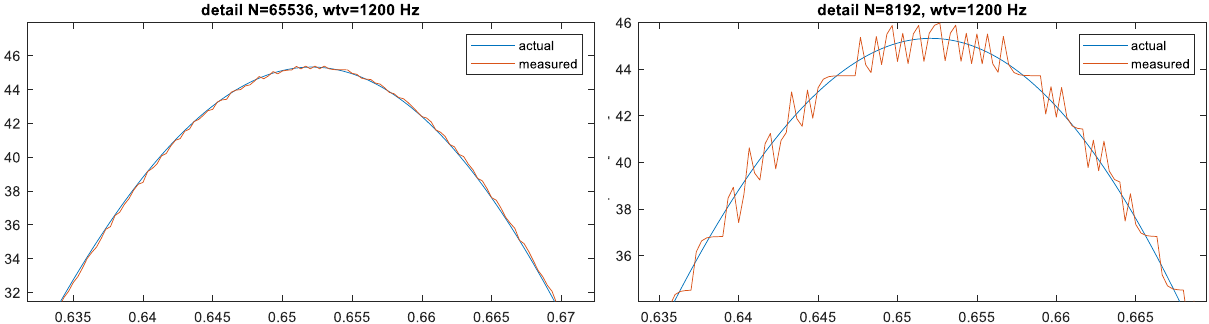
\includegraphics[width=0.8\textwidth]{Immagini/encoder1vs1_stesso_filtro.png}
    \caption{Rumore per due encoder filtrati con stesso pb}
\end{figure}

\paragrafo{Effetto del rumore:}
Il rumore che si inserisce nel ramo di feedback ritorna nel ramo di andata dove viene moltiplicato per \(K_{pv}\) (che potrebbe amplificare il rumore), filtrato dall'anello di corrente, ma non in modo sostanziale, in seguito viene moltiplicato per \(K_T\), per cui il rumore diventa un disturbo di coppia, che va al sistema meccanico, dove eccita le risonanze e il motore vibra nel gioco \footnote{Immagino il rotore che vibra quindi si muove di poco in senso orario fino a colpire l'estremo superiore del gioco e poi in senso antiorario in cui va a colpire l'estremo inferiore.}, che viene "eccitato".

Prendendo gli stessi encoder di prima, ma cercando di ottenere \textbf{parità di rumore}, quindi filtrando maggiormente per quello avente minor risoluzione e di conseguenza aumentandone il ritardo, si nota come \(K_{pv}=\frac{\omega_{b,v}^{des}J}{K_T}\) ossia \textbf{maggiore la banda passante, maggiore l'amplificazione del rumore}. Nell'esempio precedente i valori sono \(K_{pv}=1.3\) per \(\omega_{b,v}=136 \unitamisura{rd}{s}\) e \(K_{pv}=6.6\) per \(\omega_{b,v}=660 \unitamisura{rd}{s}\).

\begin{enumerate}
    \item Potrebbe andare bene lavorare con encoder più risoluto anche se l'amplificazione è elevata
    \item Potrebbe andare meglio usare l'encoder poco risoluto, alzando \(\uparrow \omega_{tv}\) e \(\uparrow\) rumore di velocità, mantenendo i guadagni limitati
    \item Potrebbe andare meglio usare l'encoder molto risoluto, abbassando \(\downarrow \omega_{tv}\) e \(\downarrow\) rumore di velocità, mantenendo un alta frequenza del polo del trasduttore di velocità
\end{enumerate}

\begin{figure}[h]
    \centering
    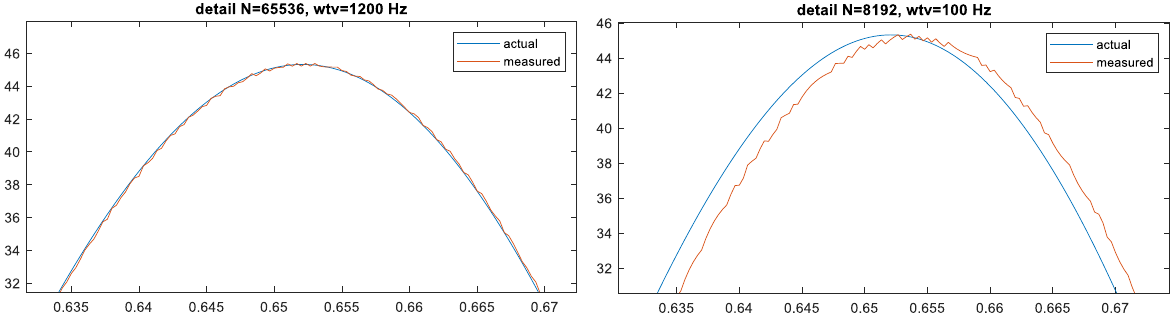
\includegraphics[width=0.8\textwidth]{Immagini/encoder1vs1_stesso_rumore.png}
    \caption{Ritardo per due encoder con stesso rumore}
\end{figure}

\sottosottosezione{Stimatore di velocità}
Derivando la posizione si ottiene una stima di velocità, che però è ottenuta utilizzando un filtro passa basso, perciò la stima è buona a bassa frequenza.
Se però si partisse da un valore di accelerazione, lo si integrasse, filtrasse con un filtro passa alto, si otterrebbe una stima di corrente buona ad alta frequenza.
L'accelerazione non viene misurata direttamente, ma si può ricavare a partire da misure di corrente (che sono influenzate dalla banda passante di corrente, che però è elevata); valgono: \(C_m=K_T i= J \AccAng + C_e\), da cui \(\AccAng = \frac{K_T i - C_e}{J}\) in cui l'unico elemento non noto è la coppia legata alle forze esterne \(C_e\).
\(C_e\) si potrebbe stimare, oppure si può assumere sia in bassa frequenza, quindi filtrando con un passa alto (come anticipato è già presente un passa alto, perciò si utilizza quello) si può attenuare.
Così facendo si ottiene una stima a ridotto rumore, ritardo e con \(\omega_{tv}\simeq \frac{2\pi f_c}{2}\)

\import{Immagini}{stimatore_velocita}

\sottosottosezione{Variazione dell'inerzia}
Tarato il controllore per \(J=J_{nom}\) e ottenuto \(K_{pv}\) tale che \(\max{m_\phi}\), variare l'inerzia può creare problemi.
Se nel sistema con quel controllore l'inerzia dovesse aumentare: \(\downarrow \omega_{b,v}^r=\frac{K_{pv}K_T}{\uparrow J}\), perciò \(\uparrow t_r\) e considerando \(\omega_{b,v}\simeq \omega_a\), \(\downarrow \omega_a\) ossia \(\downarrow m_\phi\) e \(\downarrow \xi\). L'abbassamento del fattore di smorzamento introduce oscillazioni in bassa frequenza.
Se nel sistema con quel controllore l'inerzia dovesse diminuire: \(\uparrow \omega_{b,v}^r=\frac{K_{pv}K_T}{\downarrow J}\), perciò \(\downarrow t_r\) e \(\uparrow \omega_a\), tuttavia l'aumento della pulsazione di attraversamento porta questa ad avvicinarsi a \(\omega_{tv}\), e questo porta a \(\downarrow m_\phi\) e \(\downarrow \xi\).

\begin{figure}[h]
    \centering
    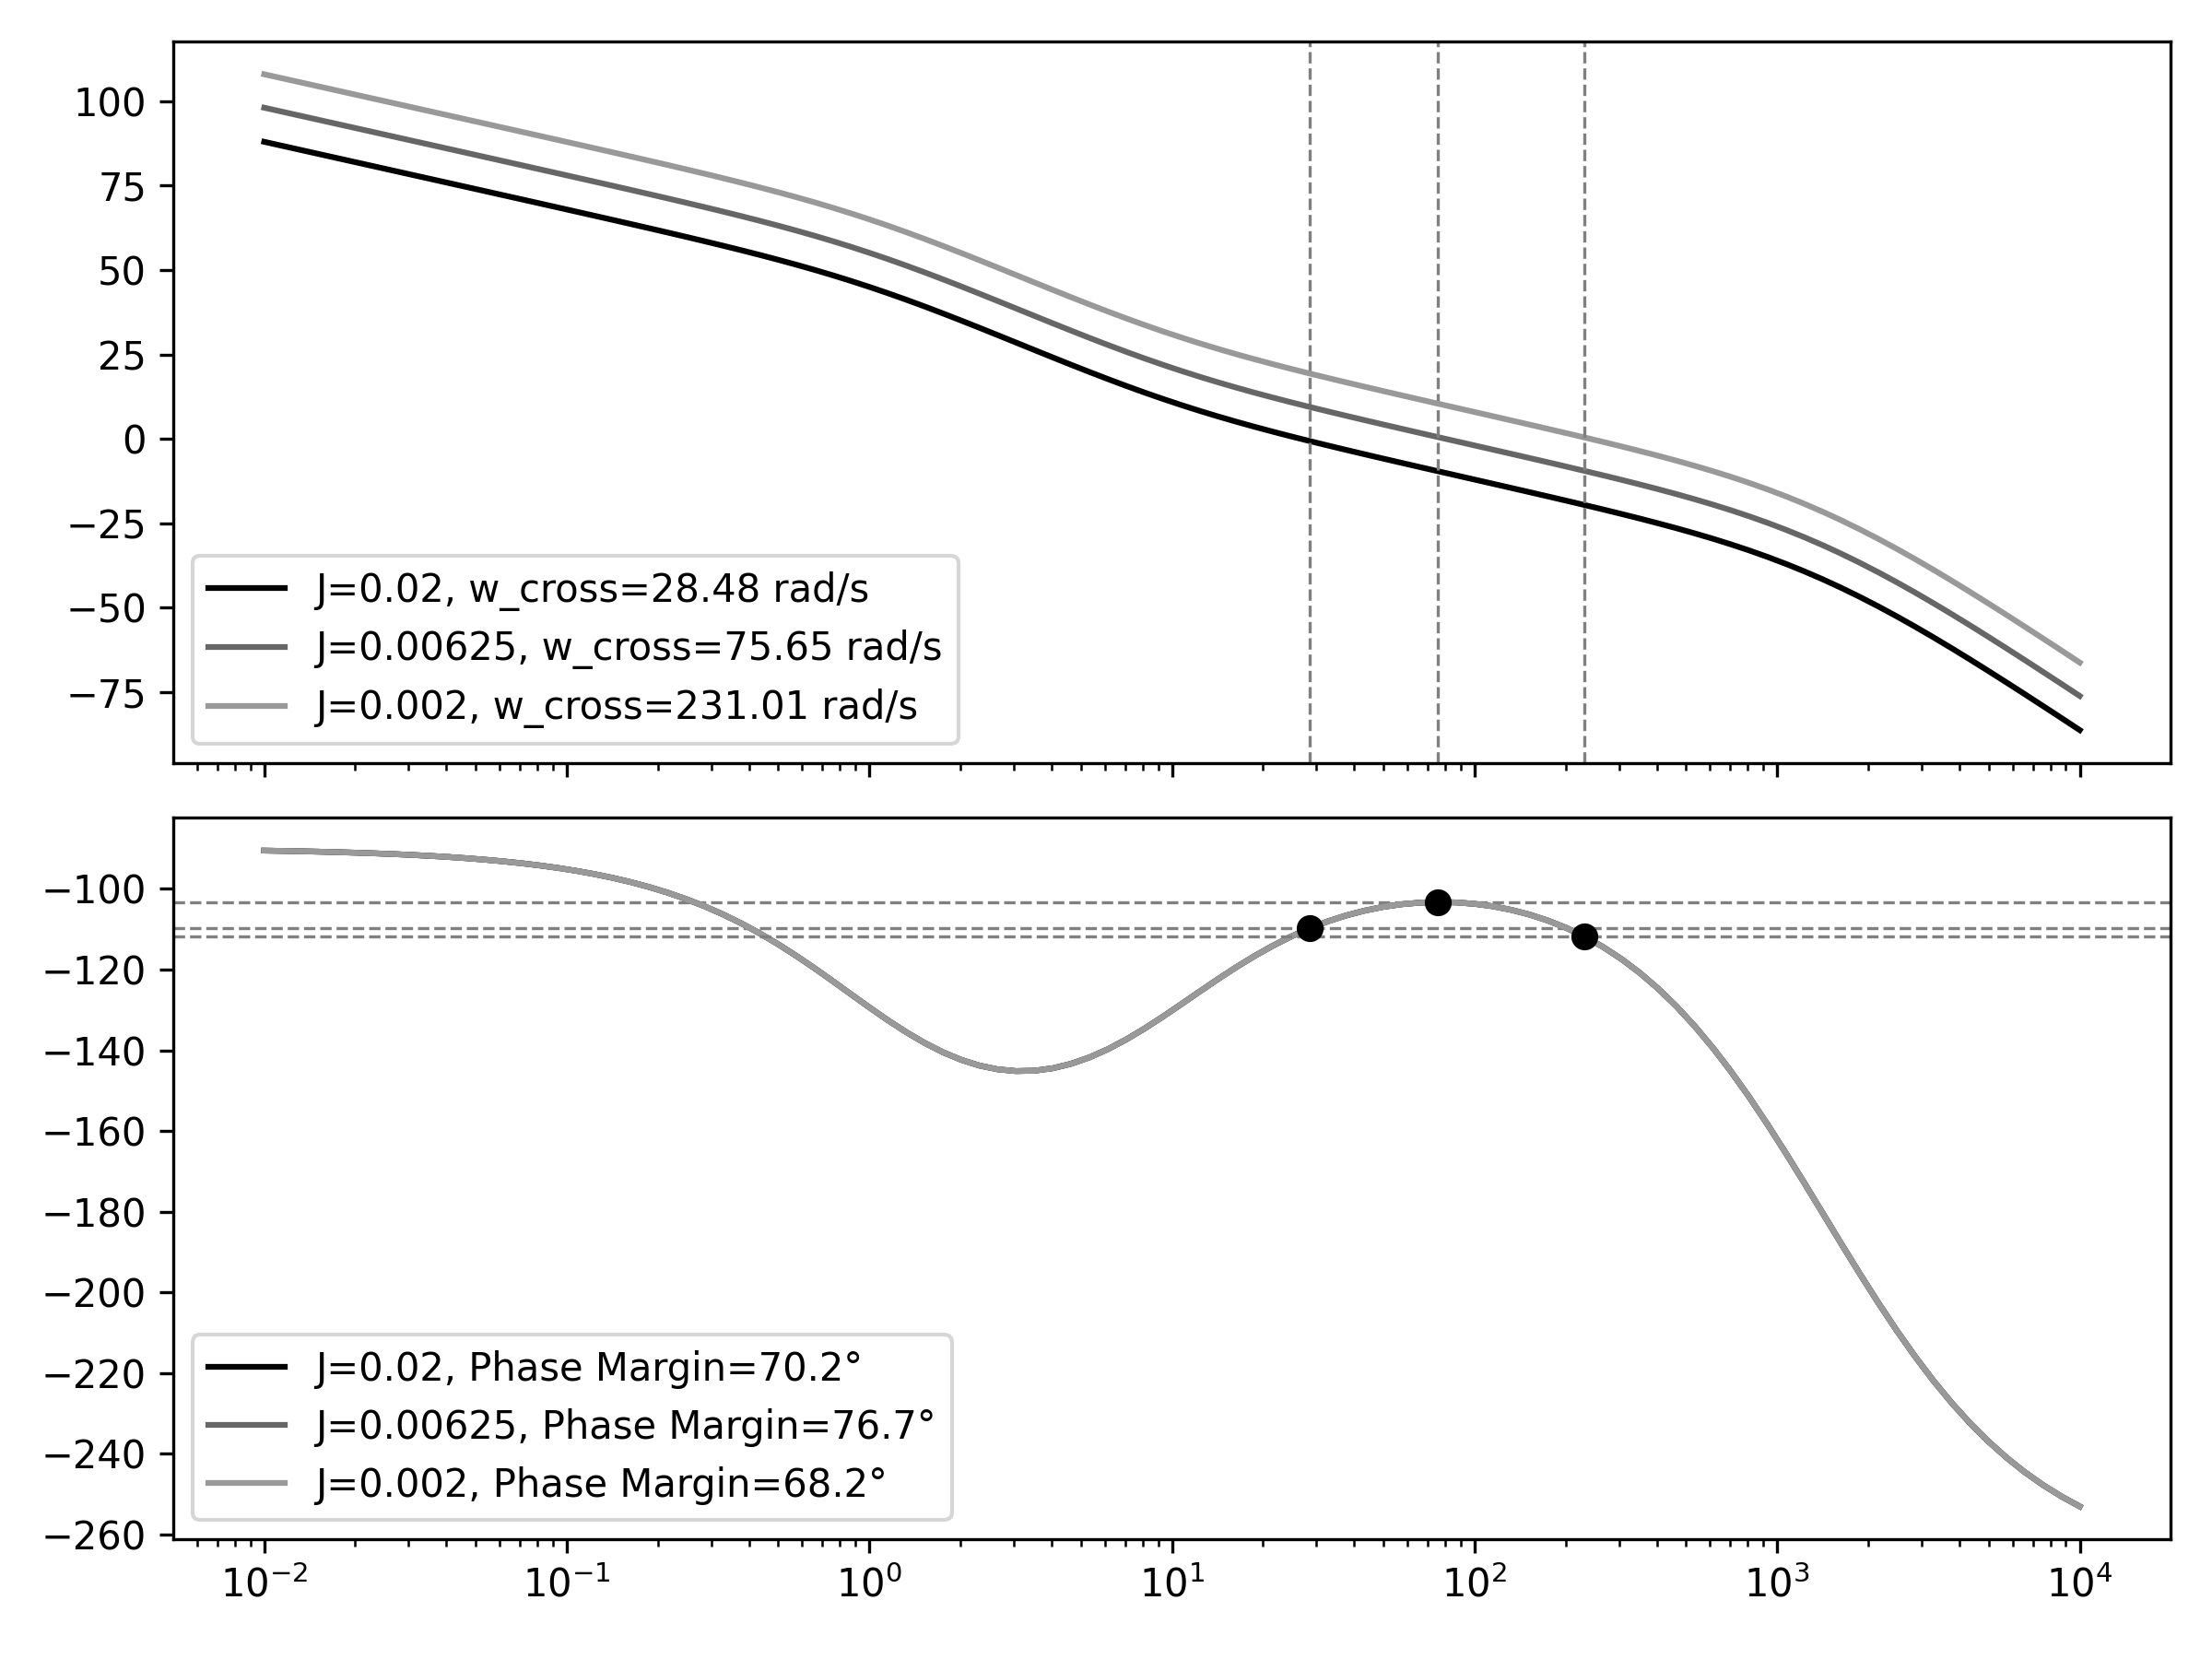
\includegraphics[width=0.6\textwidth]{Immagini/anello_velocita_J_variabile.png}
    \caption{Inerzia variabile e variazione dei parametri}
\end{figure}

\paragrafo{Gestione della variazione di inerzia con controllore "fisso":}
Per gestire la variazione di inerzia con un controllore a guadagno costante, si cerca di fare una taratura a partire da un valore di inerzia o massimo o minimo, di modo tale da assicurarsi un range di funzionamento.

\sottosezione{Feedforward}
Il feedforward aggiunto al sistema ad anello chiuso, permette di intervenire sulla \(\omega_{b,v}\) in relazione al tempo di moto e alle specifiche di inseguimento.
Ha una serie di vantaggi:
\begin{itemize}
    \item Sfrutta la conoscenza a priori
    \item Non necessita dell'errore per dare un comando
    \item Utile in transitorio
    \item Se il sistema è BIBO stabile e senza saturazione o altre non linearità, non lo destabilizza (perché opera in catena aperta)
\end{itemize}

\textbf{Il guadagno di feedforward di velocità va impostato a 1}, al controllo va passata la legge di moto com'è, di modo da poter ridurre i coefficienti del feedback e far andare il motore alla velocità progettata.
Mentre il guadagno di feedforward di accelerazione che va all'anello di coppia/corrente è il fattore di conversione tra accelerazione e coppia/corrente.

\sottosottosezione{Costruttori}
Nei controllori industriali, per la taratura del feedforward, sono utilizzate diverse funzioni, ciascuna legata ad un termine della dinamica inversa: Inerzia; Attrito; Forze costanti; Cogging Torque del motore.

Rexroth utilizza una compensazione a coppia costante, questo permette di mantenere fisso un carico sollevato. Se il carico fosse frenato, venisse scollegato il freno, collegato il motore, ma non ci fosse il feedforward, il feedback prima lascerebbe che l'oggetto scenda, per rialzarlo solo ottenuto un certo errore. Col feedforward invece, con un opportuna sincronizzazione freno motore, è possibile mantere fisso il carico.

Kollmorgen invece utilizza un riferimento di velocità per fare una compensazione di attrito e attrito viscoso.

Rockwell infine utilizza un sistema di compensazione di attrito con modello a punti di lavoro in base alla velocità, permettendo una buona stima anche per sistemi a bassa velocità e soggetti ad attrito statico.

\sottosottosezione{Compensazione Cogging Torque}
La cogging torque è una coppia resistente che varia con \(\theta\), che è problematica a basse velocità e per motori costruiti in modo approssimativo. Possibili soluzioni sono l'aumento del guadagno per permette di mantenere la velocità costante oppure la compensazione in feedforward.

\paragrafo{Costruttori:}
Kollmorgen fa un auto-taratura tramite misura puntuale di valore di coppia in riferimento alla posizione, salva tutto in una tabella e compensa in feedforward.
Un altro costruttore crea una funzione coseno con molteplicità pari al numero di espansioni polari e la porta in feedforward.

\sottosottosezione{Compensazione di forze d'Inerzia (feedforward di Accelerazione)}
Per compensare le forze di inerzia si cerca di fare \(i^{ffw}=\frac{J\AccAng^{des}}{K_T}\). Nel feedforward non è un problema fare la derivata, perché è il riferimento (potrebbe essere analitica), sicuramente non ci sono problemi di rumore.
Non si fa una compensazione totale del feedforward (circa un \(50\div 70\% J_{reale}\)), perché si predilige il feedback (dove si cerca di avere un guadagno "abbstanza alto").
La scelta del coefficiente del feedforward porta a errori di posizione:
\begin{itemize}
    \item Guadagno alto: il feedforward diventa la componente predominante, la posizione risulta in anticipo;
    \item Guadagno basso: il feedforward è una componente poco rilevante, la posizione risulta in ritardo;
    \item Guadagno giusto: non ha sovraelongazione, assomiglia al riferimento di velocità.
\end{itemize}

\begin{figure}[h]
    \centering
    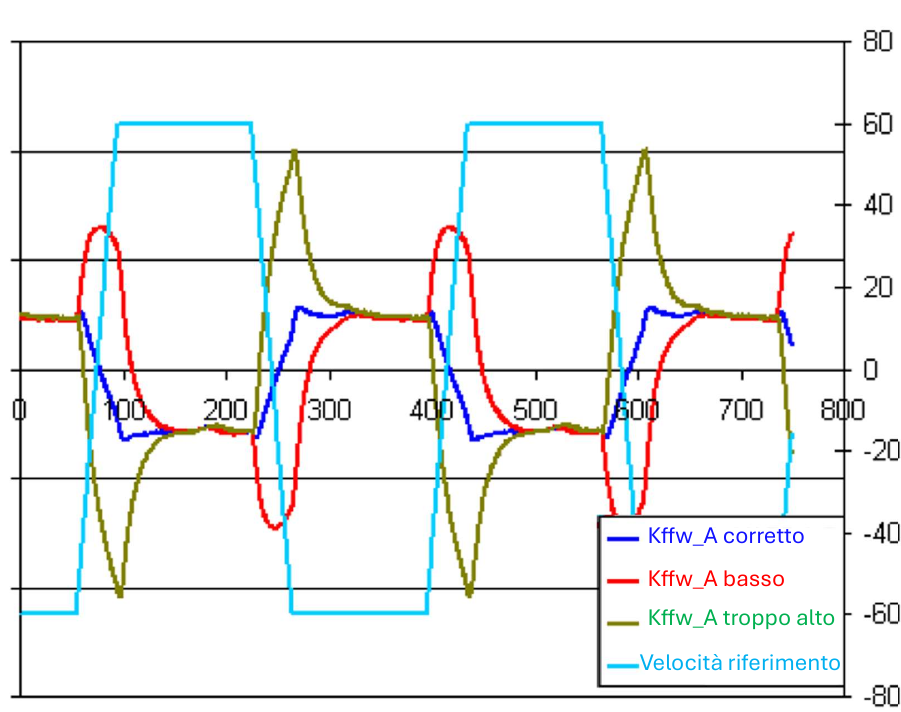
\includegraphics[width=0.5\textwidth]{Immagini/errore_posizione_feedforward.png}
    \caption{Errore di posizione per vari coefficienti di feedforward}
\end{figure}

\paragrafo{Inerzia variabile:}
Nel caso di inerzia variabile, il feedforward viene tarato su \(J_{min}\) (eventualmente per un certo fattore), così che la compensazione sia minima.


\sezione{Anello di Posizione}
Per il calcolo della velocità desiderata va fatto il calcolo col feedback, ma va aggiunto il contributo del feedforward, perché va tenuto conto il progetto della legge di moto di velocità, aggiunto col feedforward.
\(\Omega^{des}(s) = C_p(s)E_p(s) + s\theta^{des}\) dove \(C_p\) è il controllore di posizione, mentre \(E_p = \theta^{des} - \theta^{mis}\) è l'errore di posizione.

\import{Immagini/}{anello_posizione}

\paragrafo{Ipotesi semplificative:}
Per l'anello  di posizione si faranno due ipotesi semplificative: viene trascurato il trasduttore di posizione (perché \(\omega_{tp}\geqslant \omega_{tv} >> \omega_{b,v} >> \omega_{b,p}\), verranno fatte valutazioni più avanti (vedi \ref{ordine_anello_pos_vel}) su questo proposito); viene semplificato l'anello di velocità, considerando di aver ben sintonizzato l'anello di velocità (quindi scelto un buon smorzamento) \(W_v(s)=\frac{1}{1+\frac{s}{\omega_{b,v}}}\), modello che è ben rappresentato in bassa frequenza con PI (\(W_v(0)=1\) e \(\xi \simeq 1\)); viene trascurato il feedforward di velocità, che però è presente, per focalizzarsi sul feedback.

\import{Immagini/}{anello_posizione_semplificato}

\sottosezione{Controllore P}
La funzione ad anello chiuso di posizione è data da \(W_p(s) = \frac{\theta_m(s)}{\theta_m^{des}(s)} = \frac{K_{pp}\omega_{b,v}}{s^2 + s \omega_{b,v} + K_{pp}\omega_{b,v}}\). Questa funzione ha \(W_p(0) = 1\), l'errore a regime è nullo con ingresso costante/a gradino, e l'errore a regime è nullo con legge rest to rest in posizione.
Per questo motivo è sufficiente un controllore proporzionale\footnote{Aggiungere un integrale tende a introdurre problemi, ha senso solo se le forze esterne sono elevate e non prevedibili o non compensabili in feedforward.}. Questo è possibile perché c'è un integrale fisico tra velocità e posizione.

Analisi dei poli: \(\omega_{n,p} = \sqrt{K_{pp} \omega_{b,v}}\) e \(\xi_p = \frac{1}{2}\sqrt{\frac{\omega_{b,v}}{K_{pp}}}\), valgono:
\( \uparrow K_{pp} \rightarrow \begin{cases}
    \uparrow \omega_{n,p} \\
    \downarrow \xi_p
\end{cases}
\) il coefficiente proporzionale va dimensionato per limitare la sovraelongazione in posizione e \( \uparrow \omega_{b,v} \rightarrow \begin{cases}
    \uparrow \omega_{n,p} \\
    \uparrow \xi_p
\end{cases}
\) ossia l'effetto è benefico, per questo è fondamentale una buon sintonizzazione dell'anello di velocità.

Privilegiare la sovraelongazione di posizione porta ad un peggioramento di \(\omega_{b,p}\) che possono venire compensati in feedforward di velocità, che va direttamente all'anello di velocità e quindi non risente della ridotta \(\omega_{b,p}\).

\sottosottosezione{Sintonizzazione}
Per effettuare la sintonizzazione dell'anello di posizione vengono considerati \(\xi^{des}_p = 1\div 1.5\) e l'anello di velocità ben sintonizzato, perciò valgono\footnote{\(\omega_b = \omega_n \sqrt{1-2\xi^2+\sqrt{2-4\xi^2+4\xi^4}}\simeq \frac{\omega_{n,p}}{\xi} 0.65\)}:
\[\begin{cases}
    K_{pp} = \frac{\omega_{b,v}}{4(\xi^{des})^2} \\
    \omega_{b,p} \simeq \frac{\omega_{n,p}}{\xi} 0.65 \\
    \omega_{n,p} = \sqrt{K_{pp} \omega_{b,v}}
\end{cases}
\]
Unendo la prima e la terza: \(\omega_{n,p} = \frac{\omega_{b,v}}{2\xi_p}\), mentre unendo tutte: \[\omega_{b,p}\simeq \frac{0.65}{2}\frac{\omega_{b,v}}{\xi^2_p} \simeq 
\begin{cases}
    \frac{\omega_{b,v}}{3} \text{ \ se \ } \xi_p = 1 \\
    \frac{\omega_{b,v}}{6} \text{ \ se \ } \xi_p = 1.4
\end{cases}
\]
Per cui si verifica come \(\omega_{b,p} << \omega_{b,v}\). \label{ordine_anello_pos_vel}

\sottosottosezione{Costruttori}
Lenze: Propongono soluzioni per anello di corrente, velocità, posizione e utilizza una logica come quella esaminata nel corso. Propongono \(\xi_v=1\) e \(\xi_p=1.4\) come valori default. Inoltre permettono di variare il guadagno \(K_{pp}\) per le basse velocità (serve per il gioco).

Rockwell: Utilizzano uno stesso smorzamento per velocità e posizione, permettono di settare \(\xi\in [0.8; 1.5]\), utilizzano, come visto sopra la scalatura per determinare \(\omega_{b,p}\) a partire da \(\omega_{b,v}\). Propongono un controllo PI in posizione, ma l'azione integrale è posta a 0 di default.

Danaher/Kollmorgen: Permette di impostare i guadagni per i feedforward di velocità e accelerazione. Ricordare di impostare quello di velocità a 1.

Kollmorgen: Permette di effettuare gain scheduling: \(K_{p,v}(\theta,\VelAng), \ T_{i,v}(\theta,\VelAng), \ K_{pp}(\theta,\VelAng)\).

Beckhoff/Bosch: Pone un filtro in serie al feedforward di velocità, che può servire solo per leggi molto brusche come gradini e rampe (da non utilizzare). E anche un filtro in serie al feedforward di accelerazione, che però potrebbe servire per leggi brusche aventi gradini/rampe di accelerazione.

Bosch: Implementano una funzione di saturazione della corrente, nel caso in cui ci fosse un qualche tipo di problema che porta ad un incremento della temperatura di motore, che viene monitorata o stimata. In quei casi viene interrotta l'esecuzione della legge di moto, perciò è un evento che deve verificarsi il meno possibile.

B\&R: Effettuano un anticipo del feedforward per cercare di compensare una bassa \(\omega{b,v}\) o una bassa frequenza di campionamento della posizione. Tuttavia occorre prestare attenzione che questo non faccia partire prima del previsto il motore.

\paragrafo{Alternative di Feedforward di Accelerazione:}
Per effettuare il feedforward di accelerazione ci sono diversi approcci:
\begin{itemize}
    \item "Classico": approccio didattico per cui \(A^{des}=s^2 \theta^{des}\). Questo è l'approccio più sicuro, tuttavia non è coerente con \(\Omega^{des}\) in cui è presente anche la parte di feedback
    \item Beckhoff/Bosch: \(A^{des}=s\Omega^{des}=s^2 \theta^{des}+sK_{pp}(\theta^{des}-\theta^{mis})\) ossia deriva la velocità di riferimento all'anello di velocità, quindi con feedback e feedforward. Questo approccio è coerente con \(\Omega^{des}\), tuttavia è sbagliato perché è presente la derivata della misura ossia viene introdotto rumore direttamente all'anello di corrente, inoltre introduce un anello indesiderato e difficile da analizzare per la presenza del feedback, che può portare a instabilità.
    \item Beckhoff/Bosch v2: Un approccio intermedio tra quelli precedenti considera un fattore di ripartizione per i due fenomeni \(A^{des}=\alpha s^2 \theta^{des}+(1-\alpha)s\Omega^{des}\), empiricamente si ottiene ridotto rumore e sovraelongazione per effetto del feedforward per \(\alpha \in [0.7; 0.8]\).
\end{itemize}